%%
%% This is file `sample-sigconf.tex',
%% generated with the docstrip utility.
%%
%% The original source files were:
%%
%% samples.dtx  (with options: `sigconf')
%% 
%% IMPORTANT NOTICE:
%% 
%% For the copyright see the source file.
%% 
%% Any modified versions of this file must be renamed
%% with new filenames distinct from sample-sigconf.tex.
%% 
%% For distribution of the original source see the terms
%% for copying and modification in the file samples.dtx.
%% 
%% This generated file may be distributed as long as the
%% original source files, as listed above, are part of the
%% same distribution. (The sources need not necessarily be
%% in the same archive or directory.)
%%
%% The first command in your LaTeX source must be the \documentclass command.
%\documentclass[sigconf,review, anonymous]{acmart}\settopmatter{printfolios=true,printccs=false,printacmref=false}\setcopyright{none}
\documentclass[sigconf]{acmart}\settopmatter{printfolios=true,printccs=false,printacmref=false}\setcopyright{none}
\acmConference[ESEC/FSE 2020]{The 28th ACM Joint European Software Engineering Conference and Symposium on the Foundations of Software Engineering}{8 - 13 November, 2020}{Sacramento, California, United States}

\usepackage{booktabs}   %% For formal tables:
                        %% http://ctan.org/pkg/booktabs
\usepackage{subcaption} %% For complex figures with subfigures/subcaptions
                        %% http://ctan.org/pkg/subcaption
\usepackage[normalem]{ulem}
\usepackage{color}
\usepackage{listings}
\usepackage{algorithm}
\usepackage[noend]{algpseudocode}
\usepackage{cleveref}
\usepackage{multicol}
\usepackage{multirow}
\usepackage{placeins}
\usepackage{dblfloatfix}
\usepackage{amsthm}
\usepackage{makecell}
\usepackage{enumitem}
\crefformat{section}{\S#2#1#3}

\lstset{
  % basicstyle=\small\ttfamily
%   language=Scala,
  basicstyle=\footnotesize,
%   numbers=left,
  stepnumber=1,
   showstringspaces=false,
  % tabsize=1,
  breaklines=true,
  breakatwhitespace=true,
%   float,
  frame=tb,
}

\definecolor{dkgreen}{rgb}{0,0.6,0}
\definecolor{gray}{rgb}{0.5,0.5,0.5}
\definecolor{mauve}{rgb}{0.58,0,0.82}

\lstdefinestyle{myPythonStyle}{
  language=python,
%   aboveskip=3mm,
%   belowskip=3mm,
  showstringspaces=false,
  columns=flexible,
  basicstyle={\small\ttfamily},
%   numbers=none,
%   numberstyle=\tiny\color{gray},
  keywordstyle=\color{blue},
  commentstyle=\color{dkgreen},
  stringstyle=\color{mauve},
%   frame=single,
  breaklines=true,
  breakatwhitespace=true,
  tabsize=2,
}

\lstdefinestyle{numberedPythonStyle}{
  language=python,
%   aboveskip=3mm,
%   belowskip=3mm,
  showstringspaces=false,
  columns=flexible,
  basicstyle={\small\ttfamily},
  xleftmargin=2em,
  framexleftmargin=2em,
  numbers=left,
%   numberstyle=\tiny\color{gray},
  keywordstyle=\color{blue},
  commentstyle=\color{dkgreen},
  stringstyle=\color{mauve},
%   frame=single,
  breaklines=true,
  breakatwhitespace=true,
  tabsize=2,
}

\newtheorem{proposition}{Proposition}
\newtheorem{lemma}{Lemma}
%\newtheorem{theorem}{Theorem}
\newtheorem{assumption}{Assumption}

\setlength{\abovecaptionskip}{5pt}
\setlength{\textfloatsep}{5pt}
\setlength{\floatsep}{5pt}
\setlength{\intextsep}{5pt}
\setlength{\dbltextfloatsep}{10pt}
\setlength{\dblfloatsep}{10pt}
\linespread{0.98}
\setlist{leftmargin=5.5mm}

% \newcommand {\TODO}[1]{\textcolor{red}{TODO: #1}}
% \newcommand {\REV}[1]{\textcolor{blue}{#1}}
% \newcommand {\ST}[1]{\sout{#1}}

\newcommand {\TODO}[1]{\textcolor{red}{TODO: #1}}
\newcommand {\REV}[1]{#1}
\newcommand {\ST}[1]{}

%% Rights management information.  This information is sent to you
%% when you complete the rights form.  These commands have SAMPLE
%% values in them; it is your responsibility as an author to replace
%% the commands and values with those provided to you when you
%% complete the rights form.
% \setcopyright{acmcopyright}
% \copyrightyear{2018}
% \acmYear{2018}
% \acmDOI{10.1145/1122445.1122456}

%% These commands are for a PROCEEDINGS abstract or paper.
% \acmConference[Woodstock '18]{Woodstock '18: ACM Symposium on Neural
%   Gaze Detection}{June 03--05, 2018}{Woodstock, NY}
% \acmBooktitle{Woodstock '18: ACM Symposium on Neural Gaze Detection,
%   June 03--05, 2018, Woodstock, NY}
% \acmPrice{15.00}
% \acmISBN{978-1-4503-XXXX-X/18/06}


%%
%% Submission ID.
%% Use this when submitting an article to a sponsored event. You'll
%% receive a unique submission ID from the organizers
%% of the event, and this ID should be used as the parameter to this command.
%%\acmSubmissionID{123-A56-BU3}

%%
%% The majority of ACM publications use numbered citations and
%% references.  The command \citestyle{authoryear} switches to the
%% "author year" style.
%%
%% If you are preparing content for an event
%% sponsored by ACM SIGGRAPH, you must use the "author year" style of
%% citations and references.
%% Uncommenting
%% the next command will enable that style.
%%\citestyle{acmauthoryear}

%%
%% end of the preamble, start of the body of the document source.
\begin{document}

%%
%% The "title" command has an optional parameter,
%% allowing the author to define a "short title" to be used in page headers.
\title[Best-Effort Lazy Evaluation]{Best-Effort Lazy Evaluation for Python Software Built On APIs}

%%
%% The "author" command and its associated commands are used to define
%% the authors and their affiliations.
%% Of note is the shared affiliation of the first two authors, and the
%% "authornote" and "authornotemark" commands
%% used to denote shared contribution to the research.
\author{Guoqiang Zhang, Xipeng Shen}
%\email{trovato@corporation.com}
%\orcid{1234-5678-9012}
%\author{Xipeng Shen}
%\authornotemark[1]
%\email{webmaster@marysville-ohio.com}
\affiliation{%
  \institution{North Carolina State University}
  \city{Raleigh}
  \state{NC}
  \postcode{27519}
}

% \author{Lars Th{\o}rv{\"a}ld}
% \affiliation{%
%   \institution{The Th{\o}rv{\"a}ld Group}
%   \streetaddress{1 Th{\o}rv{\"a}ld Circle}
%   \city{Hekla}
%   \country{Iceland}}
% \email{larst@affiliation.org}

% \author{Valerie B\'eranger}
% \affiliation{%
%   \institution{Inria Paris-Rocquencourt}
%   \city{Rocquencourt}
%   \country{France}
% }

% \author{Aparna Patel}
% \affiliation{%
%  \institution{Rajiv Gandhi University}
%  \streetaddress{Rono-Hills}
%  \city{Doimukh}
%  \state{Arunachal Pradesh}
%  \country{India}}

% \author{Huifen Chan}
% \affiliation{%
%   \institution{Tsinghua University}
%   \streetaddress{30 Shuangqing Rd}
%   \city{Haidian Qu}
%   \state{Beijing Shi}
%   \country{China}}

% \author{Charles Palmer}
% \affiliation{%
%   \institution{Palmer Research Laboratories}
%   \streetaddress{8600 Datapoint Drive}
%   \city{San Antonio}
%   \state{Texas}
%   \postcode{78229}}
% \email{cpalmer@prl.com}

% \author{John Smith}
% \affiliation{\institution{The Th{\o}rv{\"a}ld Group}}
% \email{jsmith@affiliation.org}

% \author{Julius P. Kumquat}
% \affiliation{\institution{The Kumquat Consortium}}
% \email{jpkumquat@consortium.net}

%%
%% By default, the full list of authors will be used in the page
%% headers. Often, this list is too long, and will overlap
%% other information printed in the page headers. This command allows
%% the author to define a more concise list
%% of authors' names for this purpose.
\renewcommand{\shortauthors}{G. Zhang and X. Shen}

%%
%% The abstract is a short summary of the work to be presented in the
%% article.
\begin{abstract}
This paper focuses on an important optimization opportunity in Python-hosted domain-specific languages (DSLs): the use of laziness for optimization,
whereby multiple API calls are deferred and then optimized prior to execution (rather than
executing eagerly, which would require executing each call in isolation). In existing supports of lazy evaluation,  laziness is ``terminated'' as soon as control passes back to the host language in any way,
limiting opportunities for optimization. This paper presents Cunctator, a framework that extends this laziness to more of the Python language, allowing intermediate values from DSLs like NumPy or Pandas to flow back to the host Python code without triggering evaluation. This exposes more opportunities
for optimization and, more generally, allows for larger computation graphs to be built, producing 1.03-14.2X speedups on a set of programs in common libraries and frameworks.
\end{abstract}

%%
%% The code below is generated by the tool at http://dl.acm.org/ccs.cfm.
%% Please copy and paste the code instead of the example below.
%%
\begin{CCSXML}
<ccs2012>
 <concept>
  <concept_id>10010520.10010553.10010562</concept_id>
  <concept_desc>Computer systems organization~Embedded systems</concept_desc>
  <concept_significance>500</concept_significance>
 </concept>
 <concept>
  <concept_id>10010520.10010575.10010755</concept_id>
  <concept_desc>Computer systems organization~Redundancy</concept_desc>
  <concept_significance>300</concept_significance>
 </concept>
 <concept>
  <concept_id>10010520.10010553.10010554</concept_id>
  <concept_desc>Computer systems organization~Robotics</concept_desc>
  <concept_significance>100</concept_significance>
 </concept>
 <concept>
  <concept_id>10003033.10003083.10003095</concept_id>
  <concept_desc>Networks~Network reliability</concept_desc>
  <concept_significance>100</concept_significance>
 </concept>
</ccs2012>
\end{CCSXML}

\ccsdesc[500]{Computer systems organization~Embedded systems}
\ccsdesc[300]{Computer systems organization~Redundancy}
\ccsdesc{Computer systems organization~Robotics}
\ccsdesc[100]{Networks~Network reliability}

%%
%% Keywords. The author(s) should pick words that accurately describe
%% the work being presented. Separate the keywords with commas.
% \keywords{datasets, neural networks, gaze detection, text tagging}

%% A "teaser" image appears between the author and affiliation
%% information and the body of the document, and typically spans the
%% page.
% \begin{teaserfigure}
%   \includegraphics[width=\textwidth]{sampleteaser}
%   \caption{Seattle Mariners at Spring Training, 2010.}
%   \Description{Enjoying the baseball game from the third-base
%   seats. Ichiro Suzuki preparing to bat.}
%   \label{fig:teaser}
% \end{teaserfigure}

%%
%% This command processes the author and affiliation and title
%% information and builds the first part of the formatted document.
\maketitle

\section{Introduction}

\label{sec:intro}

Modern software is built upon APIs. Although APIs typically encapsulate highly optimized code, suboptimal usage of APIs can cause large performance degradation. Such a problem is especially common in Python programs, as Python has become the host language of many popular libraries or domain-specific languages (DSL) targeting performance-demanding tasks, such as NumPy~\cite{Walt:2011}, Pandas~\cite{mckinney2011pandas}, PySpark~\cite{Zaharia:2010}, Tensorflow~\cite{abadi2016tensorflow}, and PyTorch~\cite{paszke2017pytorch}.

Suboptimal usage of APIs typically involves a sequence of API calls. For illustration purpose, we show a simple example in Figure~\ref{fig:addEx}(a). While the code is simple, it suffers the performance flaw of a redundant temporary value: S1 creates an object and assigns it to \texttt{x}, but after \texttt{x} points to another object in S2, Python garbage collector (GC) releases the former object as it now has zero reference count. The program can be optimized by replacing the second statement with an in-place operation: \texttt{numpy.add(x, c, out=x)}. The argument \texttt{out=x} instructs \texttt{numpy.add} to reuse \texttt{x} to store the result. The optimization not only improves data locality, but also reduces memory usage. 

\begin{figure}
    \centering
    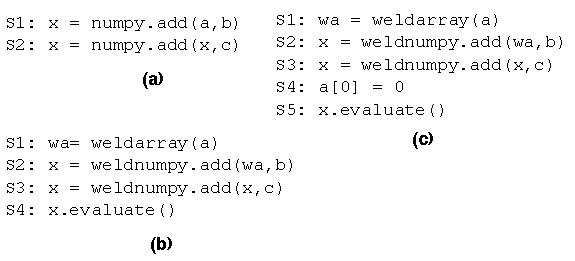
\includegraphics[width=\columnwidth]{figure/addExample.pdf}
    \caption{NumPy example and WeldNumpy variants}
    \label{fig:addEx}
\end{figure}
\begin{figure*}[t!]
    \centering
    \begin{subfigure}[c]{0.3\textwidth}
        \centering
        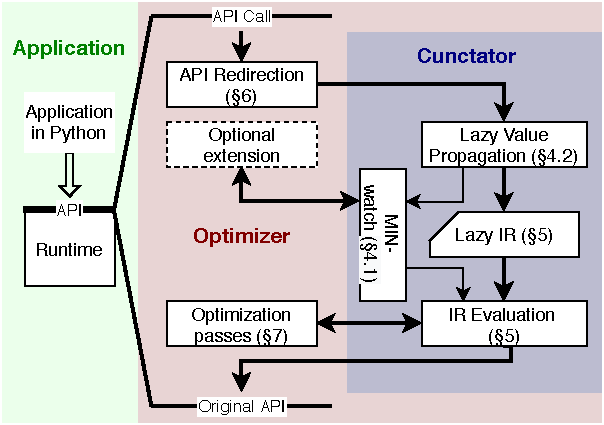
\includegraphics[height=1.8in]{figure/Overview.pdf}
        \caption{Architecture}
        \label{fig:architecture}
    \end{subfigure}
    \hfill
    \begin{subfigure}[c]{0.6\textwidth}
        \centering
        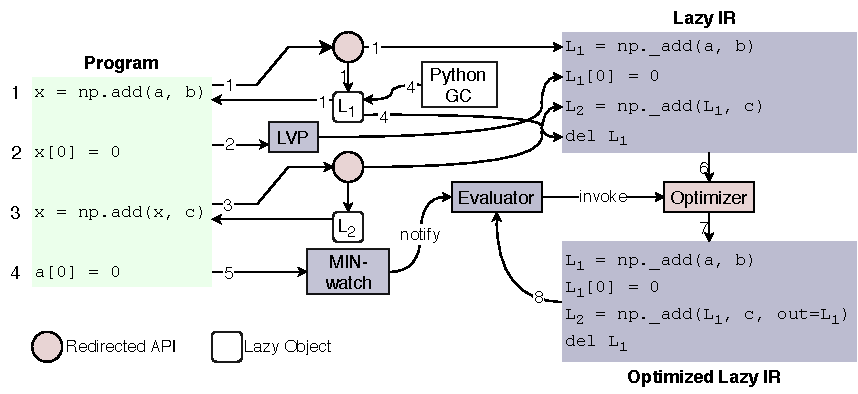
\includegraphics[height=1.8in]{figure/running_example.pdf}
        \caption{Running example. Numbers on directed edges indicate the order of actions.}
        \label{fig:running_example}
    \end{subfigure}
    \caption{Overview of Cunctator.}
    \label{fig:overview}
\end{figure*}

Existing work to tackle the problem of suboptimal API sequence relies on lazy evaluation. Several API sets, such as Spark~\cite{Zaharia:2010}, Tensorflow~\cite{abadi2016tensorflow}, and WeldNumpy~\cite{palkar2017weld}, have been designed and implemented in that way. They designate some APIs as eager APIs and the rest as lazy APIs. Invocations of lazy APIs only log the APIs in a certain form rather than execute them. Once an eager API is encountered, the logged sequence of APIs will be optimized together and then executed. For instance, Figure~\ref{fig:addEx}b shows the WeldNumpy version of the code in Figure~\ref{fig:addEx}a; the two \texttt{add} operations are not evaluated until S4; before the evaluation happens, the WeldNumpy runtime optimizes the two add operations and avoids the unnecessary object creation for \texttt{x} in the second add operation.  
%The designation is static, affected by no runtime context. 

A fundamental problem underlying the API-based lazy evaluation is the data dependence that arises between the invocations of the APIs and the host Python code. Figure~\ref{fig:addEx}c gives an illustration. Compared to Figure~\ref{fig:addEx}b, the difference is that a Python statement S4 updates the input of S1 before \texttt{evaluate()}. Python statements, by default, are eagerly evaluated. But as the \texttt{weldnumpy.add} API is lazily evaluated, S2 would end up using the wrong values of \texttt{a}.  

Existing frameworks either leave the issue to the programmers (e.g., in WeldNumpy~\cite{palkar2017weld}), relying on them to put in eager APIs at the right places, or design the library such that any API that might incur dependencies with the host code is designated as an eager API, regardless of the context (e.g., in Spark~\cite{Zaharia:2010} or TensorFlow~\cite{abadi2016tensorflow}). The former increases programmers' burdens, while the latter often misses optimization opportunities due to its conservative design.

Listing~\ref{lst:sparkagg} shows an example in {\em Spark}. It loads a text file (Line 1), splits the lines into words (Line 2), filters out illegal words (Line 3), counts the number of words (Line 4), sums the lengths of all words (Line 5), and finally outputs the average word length (Line 5). In {\em Spark}, the APIs \texttt{textFile}, \texttt{flatMap}, \texttt{filter}, and \texttt{map} are always lazily evaluated; both \texttt{count} and \texttt{sum} are always eagerly evaluated APIs \REV{because they return values to the host code and hence the value, in general, could potentially be operated on by the host code.} 
%and thus introduce dependencies, even though the result from \texttt{count} is not used in the host code before \texttt{sum} in this example code. 
When an eager API is invoked, Spark fuses relevant lazy APIs together into a pipeline; intermediate results are not cached. As there are two eager API calls, the lazy operations \texttt{textFile}, \texttt{filter}, and \texttt{flatMap} are evaluated twice at lines 4 and 5. The solution from \texttt{Spark} is to introduce extra APIs such that programmers can use them for caching. This ``band-aid'' solution further increases the burdens of programmers, who now need to be concerned of not only the usage of the many existing APIs but also the best places to use the caching APIs. 

\lstinputlisting[label=lst:sparkagg,caption=A Spark program with performance issues that are hard to automatically optimize away,float,frame=tb,style=numberedPythonStyle]{listing/spark_agg.py}

Our study (\cref{sec:eval}) shows that these limitations prevent existing frameworks from tapping into the full potential of lazy evaluations for Python+API programs, leaving up to 14X performance improvement yet to harvest. 

% The method is however subject to two important limitations.

% First, it requires compromising mechanisms to handle the dependency between a lazy API and its external operands (values not returned from lazy APIs). There are several typical solutions: (1) The lazy API makes and holds copies of the operands; (2) the operands are left unspecified as placeholders, and will be specified collectively when calling an eager API; or (3) programmers are required to invoke eager APIs at right places. The first solution introduces overheads, and other two solutions introduce programming complexity.

% Second, the static classification of eager and lazy APIs often leads to too eager executions. Take the Spark program in Listing \ref{lst:sparkagg} as an example. The program loads a text file (1), splits lines into words (2), counts the number of words (3), sums the lengths of all words (4), and finally outputs the average word length (5). APIs \texttt{textFile}, \texttt{flatMap}, and \texttt{map} are lazily evaluated; \texttt{count} and \texttt{sum} are eagerly evaluated, as their return values may be used in consequent Python operations. When an eager API is invoked, Spark fuses relevant lazy APIs together into a pipeline, thus intermediate results do not need to be cached. However, since there are two eager API calls, lazy operations \texttt{textFile} and \texttt{flatMap} are evaluated twice at lines 4 and 5.

The primary goal of this work is to create a solution that overcomes the limitations of the existing methods for enabling lazy evaluation for Python+API programming. The principles for developing our solution are two fold: (1) It should be automatic such that programmers do not need to worry about manually finding the best places in their code to insert APIs to trigger evaluations; (2) it should be effective in postponing API evaluations to places as late as possible to maximize API optimization opportunities. 

The key to both principles is to effectively analyze data dependencies between the host code and the APIs in a Python program. The problem is challenging. Many features of Python, such as dynamic typing and reflection, make analysis of the host code difficult. The difficulty is exacerbated by the extra need to analyze library APIs and their interactions with the host code. The lack of such automatic data dependence analysis is plausibly one of the main reasons for the unsatisfying solutions being used today.

In this work, we address the challenge by developing an {\em minimum interference runtime watching scheme} (MIN-watch for short). The basic idea underlying MIN-watch is simple, tracking data accesses at runtime to detect data dependencies. The novelty is in how MIN-watch makes the tracking efficient and effective for sound dependence detection in the context of Python+API programs. MIN-watch does it by taking advantage of the characteristics of Python and the special needs in lazy evaluation for Python+API. It is resilient to Python language complexities. It minimizes runtime overhead through a focused tracking scope in data and an efficient runtime checking mechanism (bit-level flagging and deferred flag resetting). It meanwhile imposes near-zero burdens on programmers. MIN-watch is based on a dependence theorem we introduce to formulate the correctness of lazy evaluation in this host+API context (\cref{sec:deps}). 
%MIN-watch exploits only two bits in the object head to achieve low overhead runtime access monitoring for Python objects. 

Based on MIN-watch, we further develop Cunctator, a software framework for materializing the extended lazy evaluation. Cunctator consists of an intermediate representation (lazy IR) for the deferred operations, a lazy IR evaluator, a class that delegates the results of deferred operations and postpones operations applied to itself, and a set of interfaces for redirecting API calls and registering optimizers. With these components together, Cunctator provides programmers the conveniences of enabling the automatic {\em Best-Effort Lazy Evaluation (BELE)} for a Python library and harvesting the optimization benefits. 

To demonstrate the usefulness of Cunctator, we implement four optimizations  enabled by BELE for three API packages (\texttt{numpy, Spark, Pandas}). Experiments on 15 programs show that the optimizations generate 1.03-14.2X speedups. Stress testing shows that the overhead of Cunctator is no greater than 2.25\% (in its default setting).

% We start with proving theorems on the conditions for finding out the latest point for lazy evaluation (\cref{sec:deps}). To leverage the theorems, a language feature of best-effort lazy evaluation (BELE) is introduced into Python (\cref{sec:bele}). BELE has two components: nested object watching for runtime dependence analysis (\cref{sec:watch}), and lazy value propagation for deferring Python operations (\cref{sec:lvp}). Built upon BELE, Cunctator is a framework that can be extended in two manners: Optimizers can be registered to manipulate the intermediate representation defined by Cunctator (\cref{sec:ir}); APIs can be augmented to leverage Cunctator through exposed interfaces (\cref{sec:apiredirect}).

In summary, this work makes the following major contributions:

\begin{itemize}
  \item It introduces the concept of Best-Effort Lazy Evaluation, and shows that MIN-watch is effective in enabling data dependence analysis for Python+API programs to support \REV{BELE\ST{Best-Effort Lazy Evaluation}}. 
  
  \item It develops the first software framework to support Best-Effort Lazy Evaluation for Python+API programs.

\item It demonstrates the effectiveness of the techniques in enabling optimizations of Python+API programs. 
    % \item To our best knowledge, we propose the first general framework targeting optimizing Python-hosted DSLs.
    
    % \item We devise an approach to perform best-effort lazy evaluation in Python. 
    
    % \item Based on our framework, we present several novel optimization techniques for Python-based DSLs.
    
    % \item We create Cunctator and evaluate its efficacy.
\end{itemize}


\section{Overview}

Figure \ref{fig:architecture} illustrates Cunctator's architecture. When an application invokes a DSL API, the API call is redirected to a Cunctator optimizer. Instead of evaluating the API, the optimizer records the API in the form of Lazy IR (\cref{sec:ir}), and returns a \textit{lazy object}. The lazy object supports  \textit{Lazy Value Propagation} (LVP, see \cref{sec:lvp}), which tries to propagate a new lazy object when an operation is applied to the lazy object. Cunctator employs MIN-watch (\cref{sec:watch}) to monitor accesses to objects related with the deferred operations. When MIN-watch encounters host statements or APIs that prevent further delays (based on dependence theorems in \cref{sec:deps}), it triggers the evaluation of the deferred operations. During the evaluation, the Cunctator optimizer applies optimization passes (\cref{sec:optimizers}) onto the IR, and then invokes the original DSL APIs for evaluation. To apply Cunctator to a domain, the developers of the DSL optimizer only needs to use Cunctator interfaces to specify redirections of the domain APIs, to support MIN-watch for some common types, and to write domain-specific optimizations. The extra work an application developer needs to do is just to import one or several modules.

% With Cunctator providing MIN-watch, LVP, IR recording, and IR evaluation,  only needs to customize the API redirection, specific optimization based on domain knowledge, and optional extension of MIN-watch. 

Figure \ref{fig:running_example} shows the execution flow of a NumPy program with Cunctator. First, the \texttt{np.add} in line 1 is redirected to Cunctator optimizer, which records the API call as a lazy IR instruction and returns a lazy object $L_1$. Note, the assignment to $x$ is not deferred but executed, and $x$ now points to the lazy object $L_1$. The optimizer also sets up the two arguments, \texttt{a} and \texttt{b}, for watching. At line 2, because \texttt{x} is lazy, the Lazy Object class automatically captures and logs this operation and defers its execution. Line 3 is similar to line 1, and Cunctator defers and logs the operation. That assignment makes \texttt{x} point to $L_2$; $L_1$'s reference count reduces to zero, which triggers Python's garbage collection on $L_1$. $L_1$'s deconstructor, however, rather than deconstructs $L_1$, defers the deconstruction and inserts a \texttt{del} instruction into the IR. Line 4 tries to update \texttt{a}, which is captured by MIN-watch, which triggers the evaluation of all the deferred operations. The evaluator first invokes the optimizer, which reduces redundant temporary variables, and then evaluates the operations.

Before presenting the details of Cunctator, in the next section, we first define some terms and prove a dependence theorem that formulate Cunctator's correctness.

\section{Dependencies between Operations}
\label{sec:deps}

To ensure the correctness of Cunctator, one key aspect is to properly manage the dependencies between postponed API calls and eagerly executed statements. We first introduce a set of terms that are used in the following discussions. 
% In other words, for any statement pair $(A, B)$ where $B$ depends on $A$, Cunctator should not postpone the execution of $A$ after $B$. In the following discussion, we first clarify and define some terms used in this section and the rest of this paper. Then, we define three types of dependencies between operations. Finally, we prove a proposition that endorses correct lazy evaluation in certain scenarios.

\vspace{0.1in}
\noindent\textbf{Terminology.} Unless otherwise stated, an \textit{object} denotes a Python object. An \textit{operator} denotes a Python built-in operator. An \textit{operation} denotes the process of applying an operator to its operands. For example, 
%\texttt{x+y} is an operation, but 
\texttt{foo.bar()} consists of two {\em operations}: The `.' {\em operator} is applied to \texttt{foo} and \texttt{"bar"} to return a function object, which becomes the operand of the `()' {\em operator}. We in addition introduce the following terms.

%\noindent \textbf{Definitions.}
\begin{itemize}
    \item \textit{Contents of an object}: All in-memory states that could be potentially accessed or updated {\em directly} through the object's fields and methods. Take the \texttt{list} object \texttt{["foo", "bar"]} as an example---its contents are the references to its two elements, the string objects, rather than the characters of the strings. By this definition, two objects could share contents, namely, their methods or attributes could access or update the same in-memory state.
    
    \item \textit{Sealed object}: An object that shares no content with other objects. This means the contents of a sealed object can be accessed or updated only by its own attributes or methods.
    
    \item \textit{Domestic object}: An object whose attributes and methods access no external resources (e.g., files and network) but only the memory space of the current process. We are interested in sealed and domestic objects (e.g., \texttt{list} objects).
    
    \item \textit{Dependents of an object}: The object itself and the objects referred to in the contents of the object. For example, the dependents of a \texttt{list} are itself and its elements.
    
    \item \textit{Relatives of an object}: The union of the dependents of that object and the dependents of its relatives.

    \item \textit{Regular operation}: An operation is regular if the relatives of its operands and return value are all sealed and domestic, and it only accesses or updates the contents of its operands' relatives or newly created objects during the operation. In most cases, a DSL API call is a regular operation.
\end{itemize}

Without noting otherwise, the following discussions assume regular operations and sealed and domestic objects and there is no exceptions. Section~\ref{sec:special} discusses exceptions and other complexities.

\vspace{0.1in}
\noindent\textbf{Dependency types.} Based on the above definitions, we classify potential dependencies between an API call $O_A$ and a statement $O_B$ into three types:

\begin{itemize}
    \item \textit{Return-access}: The return value of $O_A$ is accessed (read or written) by $O_B$, as illustrated by the top left example in Figure~\ref{fig:dependencies}.
    \item \textit{Input-update}: A relative of $O_A$'s operands is updated in $O_B$, illustrated by the bottom left example in Figure~\ref{fig:dependencies}.
    \item \textit{Update-access}: $O_A$ updates a relative of its operand $I$ and $O_B$ accesses that relative, illustrated on the right side in Figure~\ref{fig:dependencies}. Cunctator uses a conservative version of this definition, which forgoes the requirement of the two relatives being the same. It simplifies runtime checking as shown later.
\end{itemize}

\begin{figure}[htbp]
    \centering
    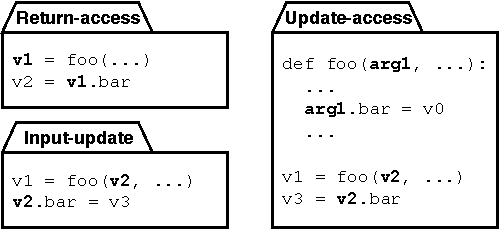
\includegraphics[width=0.8\columnwidth]{figure/dependencies.pdf}
    \caption{Three types of dependencies}
    \label{fig:dependencies}
\end{figure}

% Figure \ref{fig:dependencies} shows examples of the three types of dependencies. Note that the above definitions are pessimistic. In other words, the existence of any of these dependencies does not necessarily imply that $O_A$ cannot be deferred until after $O_B$. Take the Input-update example in Figure \ref{fig:dependencies} -- if the function \texttt{foo} never updates \texttt{v2.bar}, the two statements can be exchanged. However, their nonexistence guarantees that $O_A$ and $O_B$ can be safely exchanged in certain cases, as the following discussion justifies.

\vspace{0.1in}
\noindent\textbf{Dependency Theorem.} This part presents the dependence theorem governing the validity of lazy evaluation for APIs, which underpins the design of Best-Effort Lazy Evaluation.

\begin{lemma}
\label{lemma:dep}
For an API call $A$ followed by a statement $B$, deferring the execution of $A$ to a point after $B$ does not change the data dependencies between them if there are no {\em return-access}, {\em input-update}, or {\em update-access} dependencies between them.
\end{lemma}


The lemma comes from the observation that for the properties of sealed and domestic objects and regular operations, the three types of dependencies cover all possible data dependencies (true dependencies, anti-dependencies, output dependencies)~\cite{AK:Book} between two statements. 


\begin{theorem}
\label{theorem:dep}
For an API call $A$ followed by a sequence of statements $S$, deferring the execution of $A$ to a point after $S$ is valid if there are {\em return-access}, {\em input-update}, or {\em update-access} dependencies between $A$ and none of the statements in $S$.
\end{theorem}

This theorem is derived from the classic {\em fundamental theorem of dependence}~\cite{AK:Book}, which states the following: Any reordering transformation that preserves every dependence in a program preserves the meaning of that program. Deferring executions is clearly a kind of reordering transformation. The deferring does not cause any dependence changes according to Lemma~\ref{lemma:dep} for none of the three types of dependencies exist between $A$ and $S$. The theorem hence holds. 

Theorem~\ref{theorem:dep} is essentially a variant of the {\em fundamental theorem of dependence} in the context of API lazy evaluation; the benefits of having it are however significant. It entails what types of dependencies are needed to consider during lazy evaluation, and what set of data objects are needed to watch, which lay the foundation for the design of MIN-watch and BELE in the next section.


\section{Best-Effort Lazy Evaluation (BELE)}
\label{sec:bele}

The purpose of BELE is to defer DSL API calls until the necessary moment. The central challenge that BELE confronts is to satisfy three mutually constrained requirements: First, BELE has to ensure correctness of the program. Second, the deferring period, or \textit{laziness}, should be as long as possible to harvest optimization opportunities. Finally, the overhead should be low. 

To address these challenges, we introduce minimum interference runtime watching (MIN-watch) in \cref{sec:watch} to detect, with low overhead, \textit{input-update} and \textit{update-access} dependencies between deferred API calls and host code. In addition, Cunctator \cref{sec:lvp} employs \textit{lazy value propagation} (LVP) to manage \textit{return-access} dependencies while ensuring enough laziness. The overheads of Cunctator and strategies to control them are discussed in \cref{sec:overheadc}. Finally, \cref{sec:special} describes how to handle special scenarios.

\subsection{Minimum interference runtime watching (MIN-Watch)}
\label{sec:watch}

\begin{figure}
    \centering
    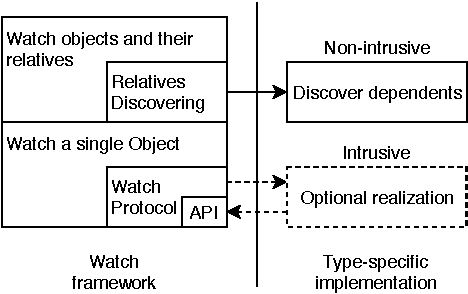
\includegraphics[width=0.7\columnwidth]{figure/watch.pdf}
    \caption{The watch framework}
    \label{fig:watch}
\end{figure}

Based on Theorem~\ref{theorem:dep}, the key for BELE is in detecting data dependencies. MIN-watch takes the way of runtime object watching, which makes it not subject to the language complexities Python imposes on compilers or other static methods. 

% To detect \textit{input-update} and \textit{update-access} dependencies for deferred operations, a natural thought is to monitor their operands. Then, once subsequent host code updates or uses a monitored operand, Cunctator triggers the evaluation of the involved deferred operations.

% Traditional methods to monitor memory access typically involve setting protection flags for relevant memory pages. However, unlike objects in static languages, a Python object does not store its contents in a continuous memory block. By default, Python stores an object's fields in a dictionary indexed by field names. But developers have the freedom to store the contents in any way they want. Such flexibility makes it difficult to figure out which memory fragments need to be monitored. Moreover, since the size of a relevant memory fragment could be far less than the page size, monitoring a lot of small memory fragments by setting their page protection flags will result in high overhead due to a high false alarm ratio.

\subsubsection{Overview of MIN-Watch}
\label{sec:overviewWatch}

What makes MIN-watch distinctive over common runtime access tracking is the strategy it employs, which takes advantage of the characteristics of this problem setting and Python language properties, and uses a lightweight type-based scheme for non-intrusive implementation. Specifically, the design of MIN-watch draws on three observations: (1) In Python, most memory accesses go through object interface with multiple layers of redirection and procedure abstractions, hence a much reduced sensitivity to runtime memory access tracking overhead compared to many other languages and settings. (2) The key to BELE is the dependence between API and host. So many data accesses that are irrelevant to such dependencies can be exempted from tracking. (3) Python object assignments and parameter passing are both through references; so to check dependencies related to an actual object, it is not necessary to track references to it, if the watching scheme is put onto that object. 

Built on the observations, MIN-watch has the following features: (1) By focusing on API to host dependencies and Theorem~\ref{theorem:dep}, MIN-watch concentrates runtime watching on only relevant data objects. (2) It employs an efficient runtime checking mechanism (bit-level flagging and deferred flag resetting) via Python interpreters to minimize interference to program executions. (3) It employs a type-based approach to enabling runtime object watching, but does it in a non-intrusive way such that application developers need to make no changes to the implementation of a data type for the approach to take effect. Moreover, the utilities in Cunctator simplify the work an optimizer developer\footnote{Please note the differences between an application developer and an optimizer developer.}
%The former writes applications in Python and some DSL APIs; the latter develops optimizations useful for optimizing applications written in the DSL APIs.} 
needs to do to enable MIN-watch (and BELE) for a domain DSL. The first two features make MIN-watch efficient, and the other features make it easy to use. 


%   The module-based scheme is general, not subject to the
%   difficulties Python poses to compilers and other static
%   analysis-based solutions. Meanwhile, it imposes almost zero extra burden
%   on application developers, who needs to make no changes to their
%   code except importing one or several modules.

%   The dependence tracking method has the following features:
%     * coarse-grained treatment to API data accesses encapsulated in
%   the augmented API module.
%     * handle both data dependencies and control dependencies
%     * robust to Python language complexities such as alias analysis,
%   dynamic types, and so on. For example, aliases to the same memory are automatically
%   addressed. In "x = numpy.add(a, b)", could x and a point to
%   the same objects? Compiler cannot handle that, but runtime checking
%   resolves that automatically)
%     * minimum sets of data tracking



% To address the aforementioned problems, MIN-watch employs a type-specific approach, which requires particular handling for each data type. While this task seems daunting, we assume that commonly used data types passed from the host code to a DSL's APIs are limited. Further, Cuncator provides a framework (Figure \ref{fig:watch}) with three features to reduce the required workload. First, the framework provides APIs to enable MIN-watch for a new type in a few lines of code. Second, the framework supports an unintrusive way to handle new types, which means the implementation of a type does not need to be changed. Finally, commonly used Python built-in types (e.g., list) are already supported.

Figure~\ref{fig:overviewWatch} uses \texttt{numpy.add(a, b)} as an example to illustrate at a high level how MIN-watch works. The API was overloaded such that when the API is called in a program, instead of doing the computation of arrays addition, it sets up objects $a$ and $b$ and their relatives for runtime watching via function \texttt{setupWatch}. Function \texttt{setupWatch} calls a function \texttt{findRelatives()} to go through each relative of an object, and calls \texttt{\_\_set\_watch\_\_} of that object to set it up for runtime watching. The setup process flags some special bits in the object header such that the extended Python interpreter, when executing a statement, can recognize such objects and invoke Cunctator lazy evaluation listener to evaluate deferred operations. 

\begin{figure}
    \centering
    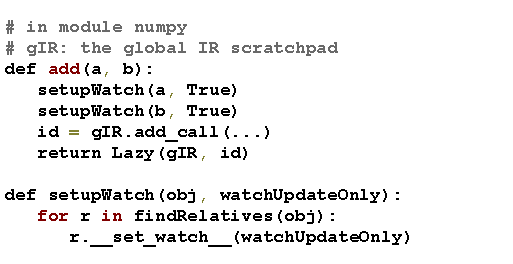
\includegraphics[width=0.8\columnwidth]{figure/watch_overview.pdf}
    \caption{A high-level illustration of how MIN-watch works for API \textit{numpy.add(a,b)}}
    \label{fig:overviewWatch}
\end{figure}

We next explain MIN-watch in detail, starting with the basic watch protocol on a single object (\cref{sec:watchproto}), and moving on to describe the procedure in finding and watching all relatives (\cref{sec:watchdeps}). 

% MIN-watch consists of two components. The basal component defines a watch protocol that can be realized by a type to support watching a single object of that type (see \cref{sec:watchproto}). Built upon the former component, the other component can watch all the relatives of an object. This is enabled through a registry that can be extended to discover dependents for specific types (see \cref{sec:watchdeps}).

\subsubsection{Watch protocol}
\label{sec:watchproto}

Cunctator adds the following method into the root class in Python: 

\begin{lstlisting}[style=myPythonStyle]
def __set_watch__(self, watchUpdateOnly):
   # pseudo-code
   self.watch_flag = WATCH_UPDATE_ONLY
   g_watch_set.insert(self)
\end{lstlisting}

The parameter \textit{watchUpdateOnly} determines whether the object should be watched for read and write accesses (\texttt{false}) or just writes (\texttt{true}).

% Any object that realizes the method should support watch. That being said, after the method's invocation, any updates or accesses (if the parameter \texttt{watchUpdateOnly} is \texttt{True}) to the object's contents should notify a global listener, which will then trigger the evaluation of lazy IR.

\begin{figure}
    \centering
    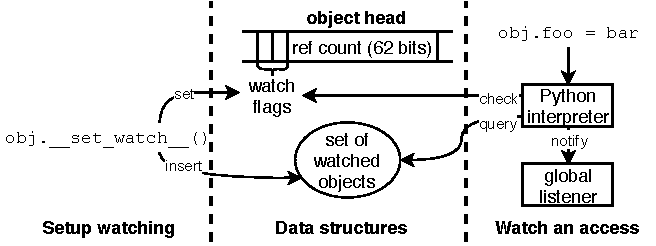
\includegraphics[width=\columnwidth]{figure/__watch__.pdf}
    \caption{Default implementation of watch protocol}
    \label{fig:watchproto}
\end{figure}

Figure~\ref{fig:watchproto} depicts the actions when the protocol takes place. In the setup time (e.g., when \texttt{numpy.add(a,b)} is called in the example in Figure~\ref{fig:overviewWatch}), \texttt{\_\_set\_watch\_\_} sets two bits in the object head to indicate whether the object is to be watched for update only (01), read/update (10), or nothing (00). These bits help the interpreter determine the corresponding action quickly. Our implementation borrows the first two bits of the reference count field of an object. That saves extra memory, and also helps ensure that most third-party binary libraries are still compatible by keeping the length of the head unchanged. The method \texttt{\_\_set\_watch\_\_} in addition adds the object into a global set \texttt{watchSet}. It is for fast resetting at the time when the deferred operations are evaluated, which will be elaborated in \cref{sec:unwatch}. 

We extend Python interpreter such that it notifies Cunctator lazy evaluation listener when the content of an object that is being watched is accessed by a bytecode (e.g., \texttt{LOAD\_ATTR} and \texttt{STORE\_SUBSCR}). 

The default implementation of \texttt{\_\_set\_watch\_\_} ignores the parameter \texttt{watchUpdateOnly} (i.e., assuming it is false). It is because when just encountering the statement, for some data types, the interpreter sometimes cannot tell whether the access would update the object. (Note that it is legitimate in Python for a seemingly read-only (e.g., \texttt{foo.bar}) operation to update the object.) This conservative implementation may reduce the laziness but won't cause correctness issues. For a given data type, the optimizer developer can choose to customize its \texttt{\_\_set\_watch\_\_()} method and other methods to enable a more precise treatment. 

% For a type that does not have that needs more precise watching to improve laziness, one could overwrite that method. The overwriting can leverage APIs provided by the watch framework; thus, the major work is to notify the listener at the appropriate time,  which typically involves only several lines of code. For example, it takes only seven lines of code to implement the overwriting for Python's built-in type \texttt{dict}.

It is worth noting that if an object is not sealed, accesses or updates to the object's contents through other objects are not watched with the default implementation. This is fixed in the upper relatives discovering component by not supporting the specific type, which causes the watch process to fail and thus triggers eager evaluations of involved operations.

\subsubsection{Watching relatives}
\label{sec:watchdeps}

With the watch protocol, we can watch a single object. MIN-watch requires watching all the relatives of an object of interest as Figure~\ref{fig:overviewWatch} has shown. The watch framework holds a registry that can register user-defined procedures to discover dependents of specific types. Through recursively calling registered procedures, all relatives of an object can be found. For example, a list $A$ contains objects $B$, $C$, and $D$, and $D$ is another list that contains $E$ and $F$. Then, the dependent-discovering procedure registered for type \texttt{list} returns $B$, $C$, and $D$ for object $A$, after which a recursive call of the procedure for $D$ returns $E$ and $F$. Typically, a type-specific dependent-discovering procedure is easy to implement. For example, the procedure for \texttt{list} is as simple as\footnote{\texttt{yield} is a Python construct that returns the next value in the next call of its enclosing function.}:

\begin{lstlisting}[style=myPythonStyle]
def list_deps(l):
    for e in l:
        yield e
\end{lstlisting}

Algorithm \ref{alg:watch} shows the process of setting up to watch an object's relatives. The \textsc{SetWatch} procedure first checks existing watch flags and returns in two cases: The first case is that the object is watched for access, when the procedure returns disregarding the parameter \texttt{watchUpdateOnly}. The second case is that the object is watched for updates only and the parameter \texttt{watchUpdateOnly} is \texttt{True}. In other cases, the procedure sets up to watch the object through the watch protocol and then recursively calls \textsc{SetWatch} for each of its dependents (except for the object itself). If the type of the object is not registered in the registry, the procedure raises an exception, which will be caught by Cunctator to trigger an eager evaluation of the involved operation.

\begin{algorithm}
\caption{Set up to watch an object's relatives.}
\label{alg:watch}
\begin{algorithmic}[1]
\State $DepReg \leftarrow $ the registry for discovering dependents
\Procedure{SetWatch}{$obj$, $watchUpdateOnly$}
%    \If {$obj$ is not watchable} throw an exception \EndIf
%    \If {$obj$ is watched}
    \If {$obj$ is watched for access} \Return \EndIf
    \If { $watchUpdateOnly \wedge obj$ is watched} \Return \EndIf
%    \EndIf
    \State $obj$.\_\_set\_watch\_\_($watchUpdateOnly$)
    \ForAll{$d \in$ \Call{Deps}{$obj$}}
        \State \Call{SetWatch}{$d$, $watchUpdateOnly$}
    \EndFor
\EndProcedure
\Procedure{Deps}{$obj$}
\If{type($obj$) is registered in $DepReg$}
\State \Return $DepReg$.getHandler(type($obj$))($obj$)
\Else
\State raise an exception
\EndIf
\EndProcedure
\end{algorithmic}
\end{algorithm}

When Cunctator defers an operation, it invokes the \textsc{SetWatch} procedure for all the operands except for lazy values, whose potential dependency is handled by lazy value propagation. 

% The parameter \texttt{watchUpdateOnly} is \texttt{False} by default. This is a conservative strategy when it is unknown whether the relatives of the operand will be updated in the operation. In many conditions, especially for DSL APIs (e.g., \texttt{numpy.add(a, b)}), we know that the operands' relatives will not be updated; thus, \texttt{watchUpdateOnly} can be set to \texttt{False}.

\subsubsection{Unwatching objects via deferred flag resetting}
\label{sec:unwatch}
After the deferred operations are triggered to get evaluated (or when a watch procedure is aborted because of an unsupported type, see \cref{sec:watchdeps}), Cunctator would need to clear the watch flags of all watched objects. Otherwise, later accesses to them would trigger unnecessary evaluations. Going through all the objects could incur substantial overhead. Cunctator circumvents it by introducing a global {\em watchSet}. Recall in Figure~\ref{fig:watchproto}, \texttt{\_\_set\_watch\_\_()} puts an object to be watched into {\em watchSet} at setup time. That set is emptied once the evaluation of deferred operations is triggered. Python interpreter, when it encounters an object with watching bits set, would check whether that object is within {\em watchSet}. If not, it cleans the watch bits; otherwise, it invokes Cunctator lazy evaluation listener. 

% \subsubsection{Special treatments}
% \label{sec:special}
%% global/static dependency

\subsection{Lazy value propagation}
\label{sec:lvp}

Return-access dependency is easy to detect for lazily evaluated operations, since all subsequent visits to the return value fall to the actually returned lazy object, which can trigger the evaluation whenever it is used, similar to how the modifier \texttt{lazy} works in some other popular languages (e.g., Scala and Swift). However, too often, a lazy object is used shortly after it is returned. For example, in the statement \texttt{(a, b) = lazy\_func()}, the lazy object is used to unpack its elements right after it is returned from \texttt{lazy\_func()}. In such cases, an evaluate-when-used semantics of lazy objects results in short-lived laziness, and leaves no optimization opportunities. As a solution to ensure sufficient laziness, we enhance Python with lazy value propagation (LVP), which propagates new lazy values for most operations applied to existing lazy values. The return-access dependency is thence not violated, since the operation that uses the return value is deferred as well.

When a lazy value is being operated, LVP records the operation into the lazy IR and then returns a newly created lazy object. One problem that LVP has to solve is when the propagation should stop -- in other words, when the true evaluation should be triggered. An evident scenario is when a lazy value is used to determine the execution branch (e.g., the \texttt{if} condition). Theoretically, we could explore all possible paths and collect the lazy IR in the form of computational tree logic (CTL)~\cite{Clarke:1981}. Such exploration, however, would introduce large overhead, while its benefit is unclear. Another situation of stopping LVP involves overhead control (see \cref{sec:overheadc}).

\lstinputlisting[label=lst:lazyclass,caption=Lazy value propagation,float,frame=htb,style=myPythonStyle]{listing/lazy.py}

Cunctator implements LVP within the class of lazy objects through operator overwriting, as shown in Listing \ref{lst:lazyclass}. A lazy object is bound with one lazy IR variable. The \texttt{\_\_add\_\_} function, for instance, overwrites the operation \texttt{lazy + r}. Their operands are set up for watching before the operation is recorded in the lazy IR. Other operations are overwritten in a similar way, except for the \texttt{bool()} operation, which triggers the evaluation, as the operation is invoked when a value is used for branch selection. Although the \texttt{bool()} operation does not necessarily imply branching, it is a good heuristic.

It is worth noting that Cunctator chooses to implement LVP in pure Python for fast prototyping. We plan to re-implement it as a part of Python interpreter in the future. \REV{This built-in LVP will have lower overhead and know precisely when a value is used for branch selection.}

\subsection{Overhead control}
\label{sec:overheadc}

If there are too many inexpensive DSL API calls or too many propagated lazy values, generating and evaluating the lazy IR could introduce too much overhead. Although such cases never appear in our experiments, we still introduce a dynamic scheme to prevent it from happening in the extreme cases. Cuncator employs a parameter $\mathcal{N}_{IRPS}$ to control how many lazy IR instructions can be generated per second. Initially, Cunctator sets a variable $\mathcal{M}$ to $\mathcal{N}_{IRPS}$. When the total number of generated instructions is equal to $\mathcal{M}$, Cunctator evaluates recorded IR, then it sets $\mathcal{M}$ to $\mathcal{N}_{IRPS} * T$, in which $T$ is the total elapsed time since the first API is deferred. If $\mathcal{M}$'s new value is smaller than its old value, it indicates that the program is an extreme case; Cunctator disables itself by avoding API redirection and LVP. In our experiments, we set $\mathcal{N}_{IRPS}$ to 1000. 

%In addition, watching too many objects causes large overhead as well. Cuncator employs a similar mechanism to control it.

%\subsubsection{Too many DSL API calls}  We currently set a limit of ten thousand for the number of API calls allowed to be captured by Cunctator. This limit covers all the DSL programs we have investigated. Based on an experiment result, lazy evaluation for ten thousand API calls costs 100\char`\~ 200ms on a modern CPU. 

%A more flexible strategy could be evaluating the lazy IR when the initial limit is reached, and then determining the next limit to fulfill an overhead target based on the time spent on evaluation. For example, let the overhead target be less than one hundred API calls per second, which means 0.1\char`\~0.2\% overhead, then after ten thousand (the initial limit) API calls are recorded, Cunctator triggers true evaluation. If the evaluation takes 1000 seconds, the next limit is set to $100\times1000 = 100,000$. If the evaluation takes less than 100 seconds, which violates the overhead target, then Cunctator is disabled and all subsequent API calls are eagerly evaluated.

%\subsubsection{Too many propagated lazy values}
%\label{sec:overheadpropa}

% In some extreme cases, lazy value propagation may cause a lot of overheads. Consider the following loop:
% \begin{lstlisting}[style=myPythonStyle,frame=tb]
% for i in range(len(a)):
%     a[i] = a[i] + lv
% \end{lstlisting}
% When \texttt{lv} is a lazy value, the loop results as many propagated lazy values as the length of array \texttt{a}. This could be a big overhead if array \texttt{a} is large. To address this problem, Cunctator sets a maximum threshold for the ratio of the number of propagated lazy values to the number of redirected DSL APIs. When the threshold is reached, no more lazy value propagation is allowed and the involved operation is eagerly evaluated.

% \subsubsection{Too many watched objects}
% \label{sec:overheadwatch}




\vspace{-.1in}
\subsection{Additional complexities}
\label{sec:special}

\vspace{0.1in}
\noindent\textbf{Exception.} Theorem~\ref{theorem:dep} assumes that neither $O_A$ nor $O_B$ raises exceptions. Exceptions could direct the execution to their handlers. If there is no exception handler set up, which is the case for most of the DSL programs we encountered, any raised exception would cause the program to crash. Thus, Cunctator disregards potential exceptions of an operation when there is no installed exception handler. When the current context has exception handlers, Cunctator disables BELE, and thence, all operations are eagerly evaluated. Cunctator checks the currently installed exception handlers through an interface added to Python interpreter.

\noindent\textbf{External dependency.} Theorem~\ref{theorem:dep} assumes that $O_A$ and $O_B$ are not dependent on each other through external resources (e.g., one writes to a file, and the other reads the file). Cunctator considers that the information of whether lazily evaluated APIs access external resources as domain knowledge and relies on the optimizer's developer to provide the knowledge. If none of the lazily evaluated operations access external resources, there is no external dependency. Otherwise, a monitor that watches the program's system calls could notify Cunctator when the program tries to access external resources; Cunctator can then avoid deferring the operations. 

\noindent\textbf{Unwatchable objects.} Although the watch framework works in most cases, there are objects that cannot be watched because they are not sealed or domestic. For example, if an object holds a segment of shared memory, an update to the shared memory in another process will not notify the listener. In addition, it is impractical to implement MIN-watch for all potential types; thus, some uncommon types may not support MIN-watch. Any kind of unwatchable object causes an involved operation to be eagerly evaluated.

\noindent\textbf{Loss of seal.} \REV{A sealed object may become not sealed at runtime. For example, \texttt{numpy.ones()} creates a sealed object \textit{O}; however, \texttt{O.reshape()} may create a new object \textit{P} that shares \textit{O}' data buffer (not a Python object) through pointer alias, rendering that \textit{O} is not sealed any more, and updates to the data buffer by operating \textit{P} cannot be monitored by watching \textit{O}. Therefore, if a type supports MIN-Watch, and there is a method of the type leaks the content, the method needs to mark the involved object as unwatchable by setting watch flags' value to 11 (see \cref{sec:watchproto}). Subsequent attempts to set watch on \textit{O} will enforce eager evaluation.}



\section{Intermediate Representation}
\label{sec:ir}

This section gives details on the design of the lazy IR in Cunctator.  
The lazy IR has a static single assignment (SSA) form. Each instruction is a 4-tuple: 
\[
<ID, OP, Operands, Annotation>
\]
$ID$ is a globally unique name, which represents the result of current instruction. $OP$ is the operator, such as `+', `.' (attribute access), `[]' (array alike access), `()' (function calls). $Operands$ are stored as a list. $Annotation$ can be used to store any extra info that the optimizer may use. For an API call, for instance, it is logged as a \texttt{call} instruction ($OP$ is `()'), the function pointer is stored in the $Operands$ field along with the function's arguments, and the API name is put into the $Annotation$ field.

An operand of an IR instruction could be either a lazy value or a non-lazy value. When an operand is a lazy value, the instruction stores its $ID$. For a non-lazy value, the instruction stores a reference to it. (In our discussion, $L_x$ denotes a lazy value, $N_x$ a non-lazy value, and $V_x$ can be any value.)

% Currently, the $Annotation$ field is only used to record the name of an API, because an API calls is logged as a \texttt{call} instructions, in which $OP$ is the function call operator `()', and the function pointer is stored in the $Operands$ field along with the function's arguments. By annotating the name, an optimizer can easily identify specific API calls. In the future, the $Annotation$ field could be extended for other purposes, such as describing the side effect of an API call. 

% Almost all IR instructions are created during redirection of API calls or lazy value propagation. One exception is the \texttt{del} instruction, which is employed to denote the end of an $ID$'s scope. The creation of \texttt{del} instruction is initiated by Python's garbage collector: When the reference count of a lazy object becomes zero, the object will be released; then, the object's deconstructor will generate a \texttt{del} instruction.

% \vspace{0.1in}
% \noindent \textbf{IR Evaluation.} The evaluation of lazy IR is triggered in any of the following conditions:
% \begin{itemize}
%     \item A lazy value is used to choose the execution branch.
%     \item A lazy value is an operand of an eagerly evaluating operation, which is caused by unwatchable operands.
%     \item The listener is notified by an update or access to a watched object.
%     \item The program is exiting.
% \end{itemize}

% Once an evaluation is triggered, first the optimizer scans and updates the IR, and then all IR instructions are executed in sequence. Theoretically, it is possible to only evaluate part of the instructions related to the corresponding condition. For example, some instructions may be unrelated to evaluating a lazy value and thus can be skipped. However, we refrain from partial evaluation for the sake of simplicity and low overhead.

%\vspace{0.1in}
%\noindent \textbf{Optimization.} 
Cunctator provides a simple interface for optimizer developers of a DSL to register optimization passes. Each optimization pass accepts a sequence of IR instructions as input, and outputs an optimized sequence. Registered optimization passes are chained in order. During an evaluation, the sequence of all recorded IR instructions since the last evaluation is passed down through all optimization passes.

% Annotation
% Implicit Input
% why not partially evaluate
%% implicit dependency between instructions



% built-in functions:
%% f-string
%% type
%% hasattr
%% print
%% str
%% repr
%% id


\section{Optimizers}
\label{sec:optimizers}
Cunctator is an enabler. By enabling BELE, it paves the way for many optimizations that are not supported by existing DSL frameworks. We have implemented proof-of-concept DSL optimizers for NumPy, Pandas, and Spark. These optimizations fall into two categories: \textit{in-language} optimization and \textit{cross-language} optimization. The in-language optimization tries to identify inefficient API uses and replace them with some other APIs of the DSL. The cross-language optimization tries to replace APIs of one DSL with APIs of another DSL. Two techniques for each category are illustrated in the following sections.

%\subsection{In-language optimization}

\subsection{Reducing temporary variables in NumPy}

\label{sec:reducenumpy}

% \begin{figure}[htbp]
%     \centering
%     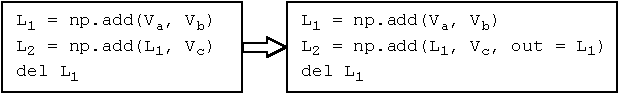
\includegraphics[width=\columnwidth]{figure/reduce_numpy.pdf}
%     \caption{Reducing redundant temporary variables in NumPy}
%     \label{fig:reducenumpy}
% \end{figure}

\begin{figure*}[ht]
\begin{minipage}[b]{0.6\linewidth}
  \centering
  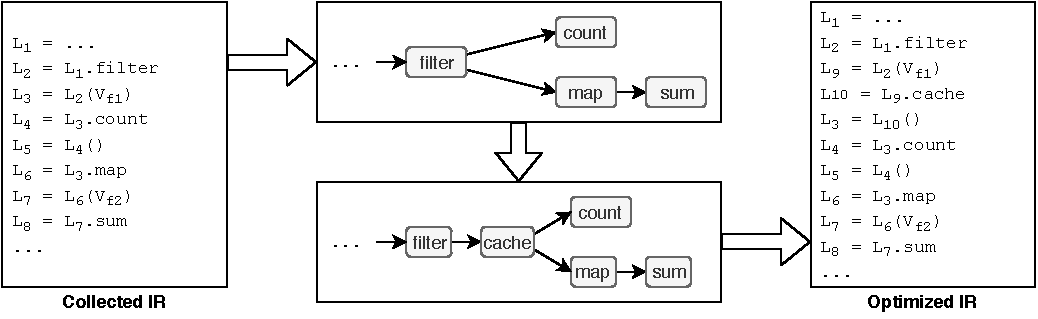
\includegraphics[width=\textwidth]{figure/merge_spark.pdf}
  \caption{Adding cache operation in Spark}
  \label{fig:sparkcache}
\end{minipage}
\hspace{0.05\linewidth}
\begin{minipage}[b]{0.3\linewidth}
  \centering
  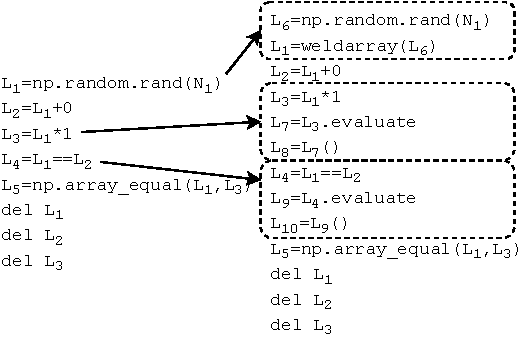
\includegraphics[trim=1 0 4 0,clip,width=\textwidth]{figure/weldnumpy.pdf}
  \caption{NumPy to WeldNumpy}
  \label{fig:weldnumpy}
\end{minipage}
\end{figure*}
% \begin{figure}[t]
%     \centering
%     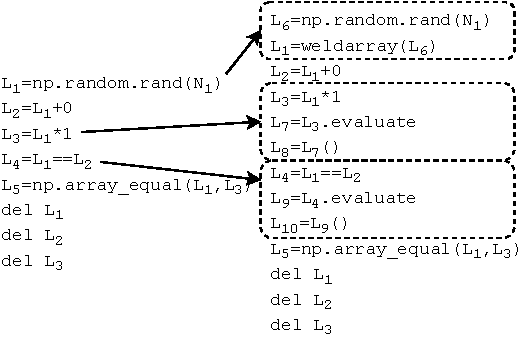
\includegraphics[trim=1 0 4 0,clip,width=\columnwidth]{figure/weldnumpy.pdf}
%     \caption{Translating NumPy to WeldNumpy}
%     \label{fig:weldnumpy}
% \end{figure}

Redundant temporary variables are a performance issue in many NumPy programs. 
%Not only because programmers may not well recognize it, but they may intentionally choose it in favour of code clarity, as the example in \cref{sec:intro} indicates.
They impair performance in two ways. First, value assignment to a new variable has worse data locality than an in-place value update. Second, depending on the array size, a temporary variable can consume a lot of memory and thus increase peak memory usage.

When the API call trace is collected as lazy IR in Cunctator, an optimizer can easily optimize away a redundant temporary variable through pattern matching and IR rewriting. At the pattern matching stage, the optimizer locates a redundant temporary variable $L_a$ if the following conditions are all satisfied:
\begin{itemize}
    \item $L_a$'s value is initialized from the result of an operation that generates a new value rather than performing in-place update.
    \item $L_a$ participates in no in-place updating operations.
    \item $L_a$ is passed to an operation $O$ that generates a new value $L_b$, and $O$ has a counterpart $O'$ that performs an in-place update.
    \item After being used in operation $O$, $L_a$ is deleted and participates in no other operations.
\end{itemize}
At the IR rewriting stage, the optimizer replaces the operation $O$ with $O'$, which saves the result to $L_a$. Figure \ref{fig:running_example} shows an example of this optimization technique.

\subsection{Adaptive caching for PySpark}

\label{sec:sparkcache}


PySpark is Spark's Python programming interface. Although Spark's runtime employs lazy evaluation to optimize its API call sequences, it fails to handle performance flaws similar to that in Listing \ref{lst:sparkagg}, because an eager API does not know whether the intermediate result of a lazy API will be used by a subsequent eager API.

With Cunctator, the performance problem in Listing \ref{lst:sparkagg} can be optimized away by adding \texttt{cache} operations for intermediate results used by more than one eager operation, as shown in Figure \ref{fig:sparkcache}. The IR shown on the left side of the figure is collected by Cunctator. Note that \texttt{del} instructions are omitted for concision. Based on the collected IR, the optimizer constructs a data flow graph for all Spark operations. If two or more eager operations share a common ancestor, the optimizer inserts a \texttt{cache} operation at the fork.

Another similar performance problem involves unnecessary \texttt{cache} operations, namely, \texttt{cache} operations for intermediate results used by only one eager API. Such operations introduce unnecessary memory writing and consume a lot of memory. Based on the same graph analysis as was used for inserting \texttt{cache} operations, the optimizer can identify and remove unnecessary \texttt{cache} operations.

\subsection{From NumPy to WeldNumpy}

\label{sec:weldnumpy}

\begin{figure}[!ht]
    \centering
    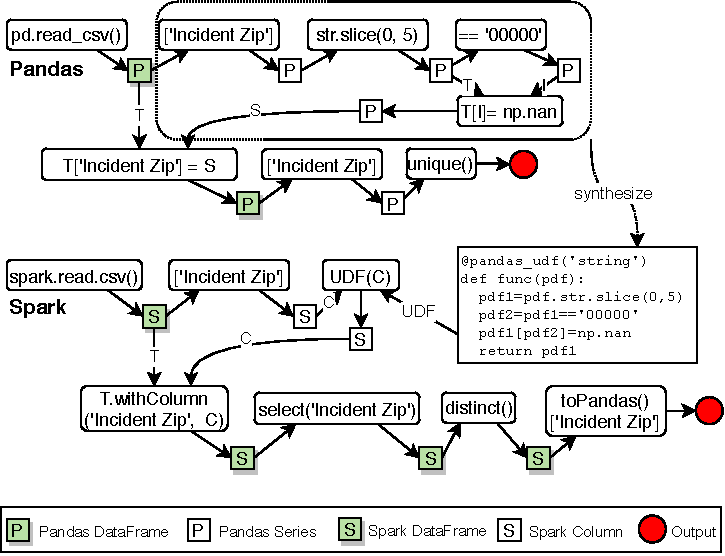
\includegraphics[width=\columnwidth]{figure/dataframe.pdf}
    \caption{Pandas to Spark}
    \label{fig:dataframe}
\end{figure}

WeldNumpy~\cite{WeldNumpy} was developed as a replacement for NumPy with better performance, which was achieved via two main techniques. First, WeldNumpy exploits lazy evaluation instead of eager evaluation, which is used in NumPy. Second, WeldNumpy implements its APIs using Weld IR~\cite{palkar2017weld}, an intermediate representation designed for parallel data processing. Through lazy evaluation, the IR fragments of invoked APIs are combined into an IR program. During a true evaluation, the IR program is compiled and optimized for native hardware. Some major optimization techniques are loop fusion, loop tiling, and vectorization. WeldNumpy provides \texttt{weldarray}, a subclass of NumPy's \texttt{ndarray}. Thus, after an \texttt{ndarray} is converted to a \texttt{weldarray}, the new object supports most NumPy operations and enjoys improved performance.

However, as WeldNumpy is lazily evaluated, it requires users to explicitly call \texttt{evaluate()} when necessary. The \texttt{evaluate()} method should not be invoked too often; otherwise, the WeldNumpy runtime misses optimization opportunities and introduces overheads of compiling the Weld IR. Neither should it be too late as that would cause errors. Thus, a NumPy-to-WeldNumpy translator needs to figure out the appropriate positions to insert \texttt{evaluate()}.

The evaluating positions can be located by identifying \textit{exposed lazy variables}. A variable is exposed if it is used beyond the DSL's APIs, which means the true value of the variable may be required, or it is alive at the end of the collected lazy IR, which allows potential external usage of the variable during subsequent execution. When a variable is exposed but lazy, it should be explicitly evaluated. Such variables can be identified within an one-pass scan of the lazy IR. The translator can thence insert \texttt{evaluate()} for these variables.

Figure \ref{fig:weldnumpy} shows an example of translating NumPy to WeldNumpy. The translated IR first converts $L_1$, an \texttt{ndarray}, to a weldarray, such that $L_2$, $L_3$, and $L_4$ enjoy WeldNumpy's optimization. However, \texttt{np.array\_equal()} is not supported by WeldNumpy; thus, operand $L_3$ has to be evaluated before being passed. While $L_4$ is explicitly evaluated because of potential exposure, $L_2$ remains lazy, since it is deleted and has no external use.

Such a translator leverages the laziness analysis enabled by Cunctator. It might be tempting to think that the translation could be done through a compiler without Cunctator. Note that that compiler would have to face the laziness analysis problem as Cunctator tackles; if it ignores that, its replacement of an eagerly evaluated NumPy API with a lazy evaluated WeldNumpy could cause errors. Doing the laziness analysis is difficult for a compiler for the many challenges (e.g., Python complexities, API-host interplay) mentioned in the introduction section. 

\subsection{From Pandas to Spark}
\label{sec:pandas2spark}

% \begin{figure*}[h]
%     \centering
%     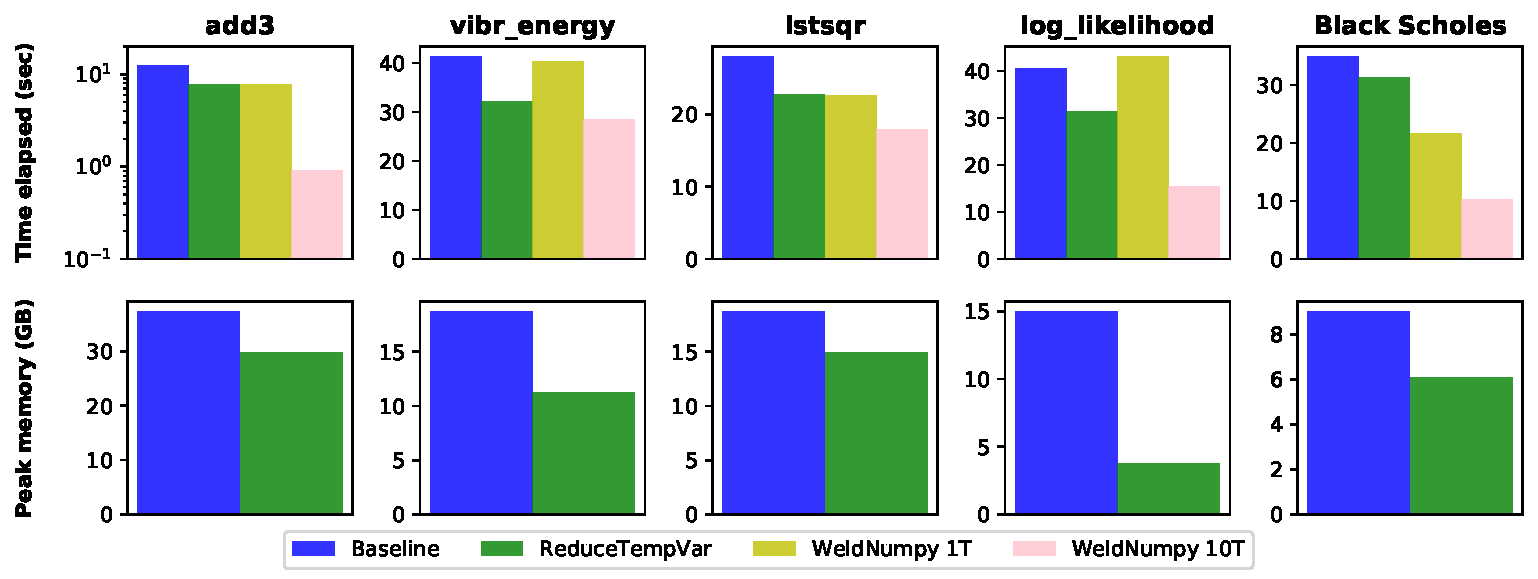
\includegraphics[width=\textwidth]{figure/numpy.pdf}
%     \caption{Optimization results of Numpy}
%     \label{fig:numpy}
% \end{figure*}

Both Pandas and Spark provide a class called \texttt{DataFrame}. They both represent logical tables, which have named and typed columns. While Pandas' operations in \texttt{DataFrame} are eagerly evaluated, most of Spark's \texttt{DataFrame} methods are lazily evaluated. During a true evaluation, Spark employs a code generation technique~\cite{Neumann:2011} to compile an operation sequence. Such technique renders the Spark DataFrame API a performant replacement of Pandas. In addition, Spark has native support for Pandas, including Pandas UDF~\cite{PandasUDF}, by which a user can apply Pandas operations to a Spark \texttt{Column}. Spark also contains type casting APIs that convert between Spark \texttt{DataFrame} and Pandas \texttt{DataFrame}. These features offers conveniences to translation of a Pandas program to a Spark program.

Similar to NumPy to WeldNumpy, the laziness analysis by Cunctator puts down the basis for the development of an automatic Pandas-to-Spark translator. Our prototype focuses on a common use pattern of Pandas: A program first loads a file as a \texttt{DataFrame}, then performs some operations on it, and finally outputs the result. In such a pattern, only one \texttt{DataFrame} object is involved, and no Pandas \texttt{DataFrame} object or \texttt{Series} (typically represents a column) object is exposed, so all instances of the two types only participate in Pandas operations. When such a pattern is matched, the translator tries to optimize it. 
%Note that the pattern is chosen to simplify our proof-of-concept prototype, but this does not imply that other patterns cannot be translated.

During the translation, the Pandas file loading function is replaced by a counterpart in Spark, thus creating a Spark \texttt{DataFrame}. Correspondingly, the \texttt{Series} objects selected from Pandas' \texttt{Dataframe} become Spark \texttt{Column} objects. If there is a sequence of operations on a \texttt{Series} that outputs another \texttt{Series}, the sequence is synthesized into a Pandas UDF for Spark, which is applied to the corresponding Spark \texttt{Column}. If a \texttt{Series} is assigned to the Pandas \texttt{DataFrame}, the corresponding \texttt{Column} is assigned to the Spark \texttt{Dataframe} as well. When an operation on a \texttt{Series} returns an object other than a \texttt{Series}, if the operation (e.g., \texttt{unique()}) has a counterpart in Spark, the \texttt{Column} is applied to the corresponding Spark operation, and then the result is converted to the expected type; otherwise (e.g., \texttt{diff()}), the \texttt{Column} is selected and converted to a \texttt{Series} before applying the operation. Figure \ref{fig:dataframe} illustrates the translation for a Pandas program collected from the Pandas Cookbook~\cite{Pandascookbook}.

\label{sec:dataframe}

% Tensorflow
%% Tuple of return values:
%%%  return (value[0], value[1])

\section{API Redirection}
\label{sec:apiredirect}

If a DSL's runtime needs to leverage Cunctator to perform optimization, the optimizer developer needs to redirect the APIs in the DSL through renaming and rewriting. With the Cunctator framework, the process is made simple. For example, to redirect \texttt{numpy.add} in NumPy's runtime, current implementation of \texttt{numpy.add} could be renamed to \texttt{numpy.\_add}; then, a new implementation of \texttt{numpy.add} will just record API calls as lazy IR instructions and returns a lazy object as shown in Figure~\ref{fig:overviewWatch}. 

To simplify the process, Cunctator offers some utilities. For the aforementioned example, what the optimizer developer needs to write to put the following into the module \textit{numpy}: 
\begin{lstlisting}[style=myPythonStyle]
def add(*args, **kwargs):
   return lazy_call("numpy.add", numpy._add, *args, **kwargs, kwargsToUpdate={"out"})
\end{lstlisting}
Method \texttt{lazy\_call} is the utility interface that Cunctator offers. Its first argument is for the annotation field of a \texttt{call} instruction (see \cref{sec:ir}). The argument \texttt{kwargsToUpdate} specifies that \texttt{numpy.\_add} is going to update only its argument \texttt{out} (if there is one). The call to \texttt{lazy\_call} in this example will essentially materialize the method shown in Figure~\ref{fig:overviewWatch}. 

\section{Efforts in Applying Cunctator}
\REV{There is some work needed from the library developers. These work needs to be done only once for a given library; the results can benefit all programs using that library. These one-time work includes: (1) redirecting some APIs that are important for performance (other APIs can be left alone, which will be treated in the same way as host Python code is); (2) supporting MIN-watch for some common types; and (3) implementing optimization passes. Table~\ref{tab:optimizers} shows our prototype optimizers' summary in these work. For a common programmer that uses a library, the only change she needs to make to her code is to insert one or several lines of code to import the optimizer.}

We initially considered automatic library transformations, but found that it was difficult to do for the complexities of Python. It is, for instance, often impossible for static code analysis to tell whether an argument is subject to modifications, due to dynamic types, aliases, higher-level functions, and inter-procedural complexities. The design choice made in Cunctator is a choice for practicability.

%For API redirection, Cunctator offers easy-to-use utility interfaces that only require several lines of code for each API (see \cref{sec:apiredirect}). It is worth noting that unredirected APIs do not affect the soundness. They are treated in the same way as host Python code is, and the data dependencies between them and the wrapped API calls are hence detected by Cunctator in the same manner.

%To support MIN-watch, a type typically only requires several lines for discovering dependents (see \cref{sec:watchdeps}). Customizing watch protocol is optional (see \cref{sec:watchproto}). In our practice, Cunctator's built-in customization of common Python types (e.g., \texttt{list}) can help harvest sufficient optimization opportunities.

%Efforts required to implement optimization passes differ in specific techniques. 

\begin{table}[htbp]
    \centering
    \caption{Summary of optimizers}
    \begin{tabular}{c c c c}
         \textbf{Optimizer} &  \textbf{\#APIs}$^*$ & \textbf{Supported types}$^\dagger$ & \textbf{Opt pass LoC}$^\ddagger$\\
    \toprule
         \multirow{2}{*}{NumPy} & \multirow{2}{*}{45} & \multirow{2}{*}{\texttt{ndarray}, \texttt{dtype}}& 50 (\cref{sec:reducenumpy})\\
          & & & 93 (\cref{sec:weldnumpy})\\
          \hline
         Spark & 24 & \texttt{RDD}, \texttt{StorageLevel} & 201 (\cref{sec:sparkcache}) \\
         \hline
         Pandas & 28 & \texttt{DataFrame}, \texttt{Series} & 436 (\cref{sec:pandas2spark}) \\
    \multicolumn{4}{l}{\footnotesize * The number of redirected APIs.} \\
    \multicolumn{4}{l}{\footnotesize $\dagger$ The types that support dependent discovery.} \\
    \multicolumn{4}{l}{\footnotesize $\ddagger$ Lines of code for implementing the optimization passes described in \cref{sec:optimizers}.}
    \end{tabular}
    \label{tab:optimizers}
\end{table}

\section{Evaluation}
\label{sec:eval}

In this section, we conduct a series of experiments to (1) demonstrate the usefulness of the four optimizations (\cref{sec:optimizers}) enabled by Cunctator, and (2) measure the runtime overhead of Cunctator. Time usage is collected by the \textit{timeit} command of jupyter~\cite{jupyter}, which adaptively chooses a number of repetitions in favor of timing accuracy. Peak memory usage is collected by \textit{memit} command extended by \textit{memory-profiler}~\cite{memoryprofiler}, which profiles a program's memory usage line by line. 
The test platform for NumPy and Pandas is a Linux machine with Intel Xeon Silver 4114 CPUs. Spark programs run on a cluster of eight Linux machines with AMD Opteron 6128 CPUs.

\subsection{Optimizers}

\begin{table*}[htbp]
  \centering
  \small
  \caption{Descriptions of collected benchmarks}
    \begin{tabular}{l|l|l|l}
    \hline
          & \multicolumn{1}{c|}{NumPy} &
          \multicolumn{1}{c|}{Spark} &
          \multicolumn{1}{c}{Pandas} \\
          \hline
    \makecell[c]{\textbf{P1} \\ Input}    &   
    \makecell[l]{Program in Figure \ref{fig:addEx}a \\ vectors of size $10^9$} &
    \makecell[l]{Program in Listing \ref{lst:sparkagg} \\ text file of 90MB}&      
    \makecell[l]{Find names of median occurrence \\ csv file of 273MB} \\
    \hline
    \makecell[c]{\textbf{P2} \\ Input}    &   
    \makecell[l]{Compute vibration energy \\ vectors of size 5×10^8 }&       
    \makecell[l]{Demultiplex a file to multiple files \\ xml file of 244MB} &
    \makecell[l]{Find top complaints \\ csv file of 526MB} \\
    \hline
    \makecell[c]{\textbf{P3} \\ Input}    &   
    \makecell[l]{Find least-squares solution \\ vectors of size 5×10^8}    &       
    \makecell[l]{Transform data format \\ json file of 62MB}&
    \makecell[l]{Find ratios of noise complaints \\ csv file of 526MB}\\
    \hline
    \makecell[c]{\textbf{P4} \\ Input}    &   
    \makecell[l]{Find log-likelihood of $\mathcal{N}(\mu,\sigma^2)$ \\ vectors of size 5×10^8}&
    \makecell[l]{Intersect IDs in two tables \\ two csv files of 34MB}&      
    \makecell[l]{Find unique zip codes after data cleaning \\ csv file of 526MB}\\
    \hline
    \makecell[c]{\textbf{P5} \\ Input}    &
    \makecell[l]{Compute Black-Scholes model \\ vectors of size 10^8}& 
    \makecell[l]{Find counts of different words \\ text file of 460MB}&     
    \makecell[l]{Find top occupations wrt. male ratio \\ csv file of 240MB}\\
    \hline
    \end{tabular}%
  \label{tab:benchmarks}%
\end{table*}%

\begin{figure*}[ht]
\begin{minipage}[b]{0.7\linewidth}
  \centering
  \small
%   \captionsetup[table]{position=bottom}
%   \captionsetup{type=table}
  \begin{tabular}{r|l|l|l|l|l}
  \hline
  & \multicolumn{1}{c|}{P1} & \multicolumn{1}{c|}{P2}  & \multicolumn{1}{c|}{P3}  & \multicolumn{1}{c|}{P4}  & \multicolumn{1}{c}{P5}  \\
  \hline
  \multicolumn{6}{c}{NumPy time usage (mean $\pm$ std. dev.)} \\
  \hline
  baseline & 12.5 s ± 2.95 ms 
           & 41.1 s ± 75.4 ms
           & 27.4 s ± 5.51 ms
           & 43.2 s ± 57.6 ms
           & 39.1 s ± 23 ms\\
  
%   w/o opt & 12.6 s ± 5.85 ms 
%           & & & & \\
  
  reduceTmp & 8.14 s ± 2.14 ms 
            & 34 s ± 15.3 ms
            & 22.9 s ± 105 ms
            & 33.7 s ± 26.9 ms
            & 32.9 s ± 22.7 ms\\
            
  Weld 1T & 6.38 s ± 34.1 ms 
          & 39.1 s ± 87.6 ms
          & 21.8 s ± 45 ms
          & 42.7 s ± 144 ms
          & 22.6 s ± 28.3 ms\\
          
  Weld 10T & 995 ms ± 9.24 ms 
           & 27 s ± 142 ms
           & 17.4 s ± 60.3 ms
           & 15.6 s ± 44.4 ms
           & 9.94 s ± 35 ms\\
  \hline
  \multicolumn{6}{c}{NumPy peak memory usage (MB)} \\
  \hline
  baseline & 38181 
           & 19131
           & 19130
           & 15316
           & 9213\\
  
  reduceTmp & 30577 
            & 11503
            & 15317
            & 3873
            & 6251\\
  \hline
  \multicolumn{6}{c}{Spark time usage (mean $\pm$ std. dev.)} \\
  \hline
  baseline & 31.9 s ± 123 ms 
           & 82 s ± 698 ms
           & 38.5 s ± 116 ms
           & 20.9 s ± 36 ms
           & 49.1 s ± 272 ms \\
           
  w/o opt & 32.1 s ± 215 ms 
          & 81 s ± 639 ms
          & 38.5 s ± 178 ms
          & 21.1 s ± 75.8 ms
          & 49.2 s ± 392 ms\\
  optimized & 17.1 s ± 93.4 ms
            & 48.8 s ± 348 ms
            & 28.8 s ± 66.8 ms
            & 20.3 s ± 317 ms
            & 47 s ± 226 ms\\
  
  
  \hline
  \multicolumn{6}{c}{Pandas time usage (mean $\pm$ std. dev.)} \\
  \hline
  baseline & 6.03 s ± 50.3 ms
           & 9.65 s ± 21.8 ms
           & 9.8 s ± 13.4 ms
           & 9.72 s ± 40.7 ms
           & 7.7 s ± 37.4 ms\\
%   w/o opt & 6.03 s ± 21.9 ms 
%           & 9.62 s ± 31.8 ms
%           & 9.82 s ± 24.9 ms
%           & 9.77 s ± 30.4 ms
%           & 7.73 s ± 23.4 ms\\
  
  Spark 1T & 17.1 s ± 100 ms 
          & 5.51 s ± 152 ms
          & 3.01 s ± 127 ms
          & 5.76 s ± 101 ms
          & 7.45 s ± 241 ms\\
          
  Spark 10T & 2.92 s ± 203 ms
          & 951 ms ± 51 ms
          & 690 ms ± 26.9 ms
          & 1.3 s ± 145 ms
          & 1.29 s ± 59 ms\\
  \hline
  \end{tabular}
  \caption{Benchmark results}
  \label{tab:results}
\end{minipage}
\hspace{0.01\linewidth}
\begin{minipage}[b]{0.28\linewidth}
  \centering
  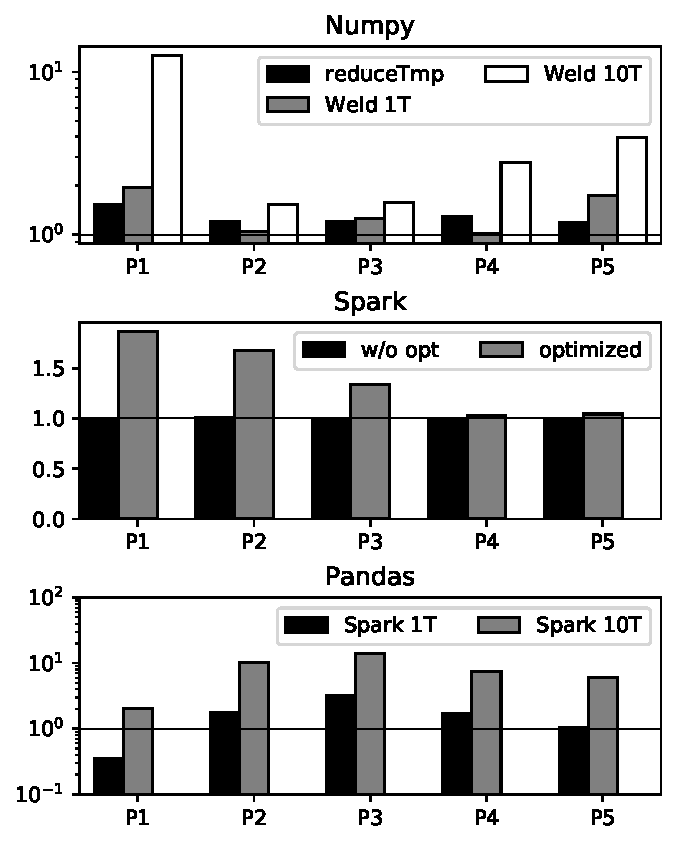
\includegraphics[width=\textwidth]{figure/speedup.pdf}
  \caption{Speedups.}
  \label{fig:speedup}
\end{minipage}
\end{figure*}

% \begin{table*}[htbp]
%   \centering
%   \small
%   \caption{Benchmark results}
%   \begin{tabular}{r|l|l|l|l|l}
%   \hline
%   & \multicolumn{1}{c|}{P1} & \multicolumn{1}{c|}{P2}  & \multicolumn{1}{c|}{P3}  & \multicolumn{1}{c|}{P4}  & \multicolumn{1}{c}{P5}  \\
%   \hline
%   \multicolumn{6}{c}{NumPy time usage (mean $\pm$ std. dev.)} \\
%   \hline
%   baseline & 12.5 s ± 2.95 ms 
%           & 41.1 s ± 75.4 ms
%           & 27.4 s ± 5.51 ms
%           & 43.2 s ± 57.6 ms
%           & 39.1 s ± 23 ms\\
  
% %   w/o opt & 12.6 s ± 5.85 ms 
% %           & & & & \\
  
%   reduceTmp & 8.14 s ± 2.14 ms 
%             & 34 s ± 15.3 ms
%             & 22.9 s ± 105 ms
%             & 33.7 s ± 26.9 ms
%             & 32.9 s ± 22.7 ms\\
            
%   Weld 1T & 6.38 s ± 34.1 ms 
%           & 39.1 s ± 87.6 ms
%           & 21.8 s ± 45 ms
%           & 42.7 s ± 144 ms
%           & 22.6 s ± 28.3 ms\\
          
%   Weld 10T & 995 ms ± 9.24 ms 
%           & 27 s ± 142 ms
%           & 17.4 s ± 60.3 ms
%           & 15.6 s ± 44.4 ms
%           & 9.94 s ± 35 ms\\
%   \hline
%   \multicolumn{6}{c}{NumPy peak memory usage (MB)} \\
%   \hline
%   baseline & 38181 
%           & 19131
%           & 19130
%           & 15316
%           & 9213\\
  
%   reduceTmp & 30577 
%             & 11503
%             & 15317
%             & 3873
%             & 6251\\
%   \hline
%   \multicolumn{6}{c}{Spark time usage (mean $\pm$ std. dev.)} \\
%   \hline
%   baseline & 31.9 s ± 123 ms 
%           & 82 s ± 698 ms
%           & 38.5 s ± 116 ms
%           & 20.9 s ± 36 ms
%           & 49.1 s ± 272 ms \\
           
%   w/o opt & 32.1 s ± 215 ms 
%           & 81 s ± 639 ms
%           & 38.5 s ± 178 ms
%           & 21.1 s ± 75.8 ms
%           & 49.2 s ± 392 ms\\
%   optimized & 17.1 s ± 93.4 ms
%             & 48.8 s ± 348 ms
%             & 28.8 s ± 66.8 ms
%             & 20.3 s ± 317 ms
%             & 47 s ± 226 ms\\
  
  
%   \hline
%   \multicolumn{6}{c}{Pandas time usage (mean $\pm$ std. dev.)} \\
%   \hline
%   baseline & 6.03 s ± 50.3 ms
%           & 9.65 s ± 21.8 ms
%           & 9.8 s ± 13.4 ms
%           & 9.72 s ± 40.7 ms
%           & 7.7 s ± 37.4 ms\\
%   w/o opt & 6.03 s ± 21.9 ms 
%           & 9.62 s ± 31.8 ms
%           & 9.82 s ± 24.9 ms
%           & 9.77 s ± 30.4 ms
%           & 7.73 s ± 23.4 ms\\
  
%   Spark 1T & 17.1 s ± 100 ms 
%           & 5.51 s ± 152 ms
%           & 3.01 s ± 127 ms
%           & 5.76 s ± 101 ms
%           & 7.45 s ± 241 ms\\
          
%   Spark 10T & 2.92 s ± 203 ms
%           & 951 ms ± 51 ms
%           & 690 ms ± 26.9 ms
%           & 1.3 s ± 145 ms
%           & 1.29 s ± 59 ms\\
%   \hline
%   \end{tabular}
%   \label{tab:results}
% \end{table*}

% \begin{figure*}[!ht]
%     \centering
%     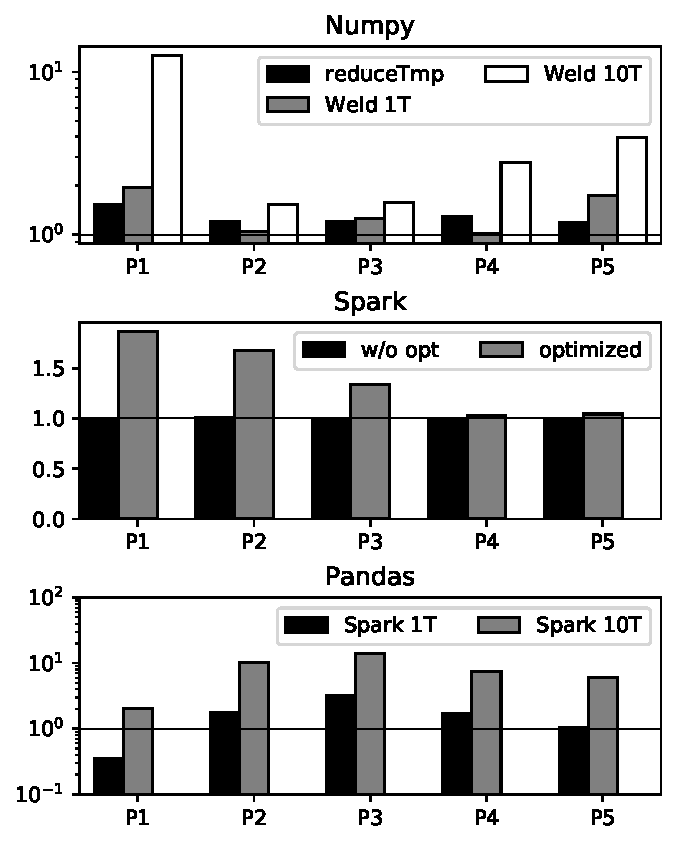
\includegraphics[width=\textwidth]{figure/speedup.pdf}
%     \caption{Speedups}
%     \label{fig:speedup}
% \end{figure*}

We collect 15 programs for the experiments that are rele-vant to the example optimizations described in the previous section; five for each of the three packages (NumPy, Spark, Pandas). Thirteen of them were collected from Github; the other two were the examples used in the earlier sections of this paper---we included them to show the performance benefits from the described optimizations. Table \ref{tab:benchmarks} shows the descriptions and inputs of all benchmarks. Figure \ref{fig:speedup} shows the speedups in different optimizer settings. Detailed results are presented in Figure \ref{tab:results}. Each program set is discussed separately in following subsections.

%For each optimizer, we collect from Github five programs that the optimizer can identify optimization opportunities. The two NumPy optimizers share the same set of benchmarks, such that their results can be compared. 


\subsubsection{NumPy}

The temporary variable reducer (abbr. \textit{reduceTmp}) accelerates all benchmarks, with speedups ranging from 1.19X to 1.54X. The highest speedup is achieved on P1, because its operations are easy to compute and hence the cost of temporary variable is prominent. Besides time benefits, \textit{reduceTmp} also reduces peak memory usage. P4 highlights the reduction with a rate of 75\%. The high rate is because of pipelined operations, which means each temporary variable is only used one time and then discarded.

For WeldNumpy converter, we test it with one thread (abbr. \textit{Weld 1T}) and ten threads (abbr. \textit{Weld 10T}) separately. \textit{Weld 1T} shows speedups ranging from 1.01X to 1.95X. Because WeldNumpy currently supports only a limited number of NumPy APIs, for unsupported APIs, it needs to transform data from Weld format to NumPy format to perform the operations, and if necessary, the results need to be transformed back. As WeldNumpy evolves to support more APIs, \textit{Weld 1T} is going to perform better. Moreover, with ten threads, WeldNumpy achieves significant speedups up to 12.5X. Note that Weld has built-in support for multi-threading but NumPy does not.

\subsubsection{Spark}

The Spark optimizer shows speedups ranging from 1.03X to 1.87X. Among the benchmarks, P1 and P2 lack \texttt{cache()}; P3 and P5 have unnecessary \texttt{cache()}; P4 has a \texttt{cache()} operation at a useless location, while the place that needs \texttt{cache()} does not have one. Our optimizer fixes them all. It adds \texttt{cache()} to P1 and P2, removes \texttt{cache()} from P3 and P5, and corrects P4 by removing the unnecessary \texttt{cache()} and adding one at the appropriate place.

In addition, we test the benchmarks with Cunctator enabled but optimizing pass disabled(abbr. \texttt{w/o opt}). The results show no performance degradation. This confirms that MIN-watch has almost no overhead for non-watched objects, as PySpark programs typically invoke user defined functions written in Python frequently.

\subsubsection{Pandas}

The Pandas-to-Spark optimizer is tested with one Spark thread (abbr. \texttt{Spark 1T}) and ten Spark threads (abbr. \texttt{Spark 10T}). Note that Spark supports multi-threading but Pandas does not. \texttt{Spark 1T} shows speedups on three programs. This is impressive because, while Pandas enjoys the high performance of SIMD instructions, Spark's query compiler emits Java bytecode. The slowdown on P1 is dominated by Spark's CSV loader, which performs much worse than Pandas' loader in this case. Nevertheless, \texttt{Spark 10T} enjoys speedups as high as 14.2X on all benchmarks.

\subsection{Overheads}

For programs cannot be optimized, a major concern is the overhead, which is highly related to the number of lazy IR instructions recorded. To investigate the overhead in different cases, we design an adversarial case for stress-testing:

\begin{lstlisting}[style=myPythonStyle, label=lst:cps_emulator]
def cps_simulator(M, N):
   for i in range(M):
      numpy.ones(N)
\end{lstlisting}

The program calls $M$ times of \texttt{numpy.ones(N)}, which initializes a vector of size $N$. By tuning $M$ and $N$, we can control the number of calls per second (CPS) and the total run time. We then combine some representative values of CPS and overhead control thresholds (see \cref{sec:overheadc}). For each combination, we run a ten-second experiment with Cunctator. By substracting the results with corresponding baseline results, we obtain an overhead matrix, shown as Table \ref{tab:matrix}.

\begin{table}
    \centering
    \small
    \caption{Overhead (percentage of 10s program runs)}
    \begin{tabular}{c r| c c c c c}
    & & \multicolumn{5}{c}{CPS}\\
     &   & 50 & 500 & 1000 & 2000 &  10000 \\
     \hline
    \multirow{5}{*}{\rotatebox{90}{Threshold}} 
    %& 10 & 0.2 & 0.5 &  0.55 & 0.95 & 0.16 & 0 \\
    & 50 & 0 &  0.85 & 0.85 & 1.7 & 0 \\
    & 500  & 0.35 & 3.05 & 1.05 & 1.8 & 0 \\
    & \textbf{1000}  & \textbf{0.25} & \textbf{2.35} & \textbf{2.25} & \textbf{1.7} & \textbf{0}\\
    & 2000 & 0.15 & 2.15 & 2.05 & 2.5 & 0.1\\
    & 10000 & 0.15 & 1.25 & 1.75 & 2.9 & 11.8\\
    \end{tabular}
    \label{tab:matrix}
\end{table}

The overhead increases when CPS increases. When CPS exceeds the threshold, Cunctator disables itself for the later part of the run; the overhead drops. For the default threshold (1000), the worst overhead is 2.35\%, which happens in the extreme case where there are 1000 function calls per second. In practice, a program is unlikely to have a stable CPS rate close to the threshold, thus the overhead is much lower. In addition, it is worth noting that Cunctator is mainly implemented in Python, except for the MIN-watch. If we reimplement some critical components in C, such as lazy IR evaluator, a lower overhead is expected.

\REV{It is worth noting that, in the domains that we explored, the number of relatives per object is few, hence our benchmarks bear little overhead of finding relatives. For example, a NumPy array usually has no relative if its buffer belongs to itself, or only one relative if its buffer is from another object. For domains where deeply nested objects are common, the overhead control threshold can be adjusted to fit the need of the domains.}

\subsection{Threats to Validity}

\REV{Cunctator is evaluated based on Python 3.7.3, NumPy 1.17.0, WeldNumpy 0.0.1, Pandas 0.25.0, and Spark 2.4.3. The APIs and implementation of these software packages may change after new versions are released. Thus the new releases may invalidate our optimization techniques and evaluation results. Nevertheless, new patterns of API misuses related to these new releases are likely to appear. Unless the new versions employ a technique similar to BELE, Cunctator can be leveraged to optimize the new patterns.}

\section{Related Work}

Lazy evaluation has been studied extensively in functional programming~\cite{Henderson:1976,Johnsson:1984,bloss1988code,Launchbury:1993,Hudak:2007}. Scala~\cite{odersky2014unifying} provides a \texttt{lazy} keyword to express the call-by-need semantics of a variable. However, Scala does not manage the potential side-effect of a thunk, the expression bound to the lazy variable; thus, the correctness of lazy evaluation relies on the programmer. Many hosted DSLs (e.g., Spark~\cite{Zaharia:2010} and Tensorflow~\cite{abadi2016tensorflow}) employ lazy evaluation; their limitations have been discussed in \cref{sec:intro}. 

% proposes an IR for parallel data processes. If a DSL's data processing APIs are rewritten in Weld IR instructions, the IR program can then be compiled and optimized to run on various hardware. Weld does not give support of best effort lazy evaluation, but rely on programmers to insert eager evaluation APIs. 

% is under the hood of DSLs' APIs, which means it relies on but is restricted by eagerly evaluated APIs. Our work, on the other hand, has a holistic view of the program and thus can break the barriers between eagerly evaluated APIs.

There are some studies on optimizing DSLs. Weld~\cite{palkar2017weld} and its limitations have been discussed and compared with. 
Delite~\cite{Sujeeth:2014} is a framework for developing Scala-hosted DSLs by leveraging generative programming~\cite{Czarnecki:2000}. Similarly to Cunctator, it lazily evaluates DSL operations and logs them as a form of IR, which will be optimized and executed at a certain point in time. However, Delite provides no mechanism to handle the dependencies between DSL operations and their host code.

There are several earlier studies (e.g., telescoping languages~\cite{telescoping}, Broadway~\cite{Broadway}) that try to use manual annotations of libraries to help optimizations. They give no systematic considerations of the host-API dynamic dependencies. Numba~\cite{Lam:2015} is a JIT compiler of Python that targets optimizing manipulations of ndarray in NumPy. AutoGraph~\cite{AutoGraph} employs static code conversion and generative programming to tranform PyTorch-style programs to Tensorflow-style programs. All these methods and tools offer a closed set of optimization techniques for specific program semantics. Cunctator does not include any optimization technique but provides a general framework to simplify the creation of a DSL optimizer.


% \section{Future Work}



% In the current prototype, Cunctator generates and evaluates lazy IR but leaves IR optimization entirely to a customized DSL optimizer. As we implement optimizers for different DSLs, we find that support for some common optimization tasks within Cunctator would be helpful. Examples include dead code elimination, common sub-expression elimination, type inference, IR pattern matching, etc. Many of these tasks require knowledge about DSL APIs. For example, to eliminate dead API calls, the optimizer needs to know whether an API call has a side effect. To obtain such domain-specific knowledge, Cunctator could allow optimizer developers to express it through an interface description language.

% Another future improvement to Cunctator involves rewriting its lazy evaluation engine in C as an extended feature of Python. Such a refactoring not only reduces Cunctator's overhead, but can also provide a more accurate call-by-need mechanism, as we discuss in \cref{sec:lvp}.


\section{Conclusion}

This paper introduces the concept of BELE, and describes MIN-watch, the first efficient runtime monitoring method tailored to data dependence analysis between host code and APIs for BELE. The paper demonstrates the usefulness of Cunctator in enabling four optimizations that are not supported by existing frameworks, giving 1.03-14.2X speedups. While Cunctator targets Python-hosted DSLs, we believe the potentially applicability of the techniques goes much beyond Python. 

%%
%% The next two lines define the bibliography style to be used, and
%% the bibliography file.
\balance
\bibliographystyle{ACM-Reference-Format}
\bibliography{references}

%%
%% If your work has an appendix, this is the place to put it.


\end{document}
\endinput
%%
%% End of file `sample-sigconf.tex'.
